

\chapter{Heating-Cooling Asymmetry: Continuous-Variable Case}\label{cap:results-continuous}

Continuous-variable (CV) systems are described by observables with continuous spectra, typically associated with infinite-dimensional Hilbert spaces. An important subclass of CV systems are Gaussian states and operations, as they have been widely applied in communication protocols, quantum field theory, solid state physics, and open quantum systems \cite{adesso-2016}. In Sec. \ref{sec:gaussian}, we present the basic theory of Gaussian systems and the main references for this section are \cite{adesso-2016, serafini-book}. In this work, we will investigate the heating-cooling asymmetry for the three cases of Gaussian states: thermal states (Sec. \ref{sec:result-thermal}), displaced states (Sec. \ref{sec:result-displaced}), and squeezed states (Sec. \ref{sec:result-squeezed}). As before, we will use the thermal kinematics approach to understand the asymmetry, however, we will use the Wigner-Fisher information instead of the quantum fisher information, which will result in some small changes on the thermal kinematics variables, which will be discussed in Sec. \ref{sec:thermo-gaussian}


\section{Gaussian States}\label{sec:gaussian}

% Quantisized fields and canonical operators 
% Phase-space, characteristic functions and quasi-probabilities distributions
% Gaussian states: mean vector and covariance matrix
% Gaussian operators: displacement and squeezing
% Ergotropy
% Wigner relative entropy
% Wigner entropy

 
An important example of CV systems is the quantised electromagnetic field, whose modes behave as independent harmonic oscillators. Despite being described by continuous variables, the energy of each mode is quantised in equally spaced levels, with transitions occurring through the absorption or emission of energy quanta known as photons. For simplicity, let us consider an electromagnetic field inside an optical cavity, where only $N$ relevant modes are taken into account. In this case, the Hamiltonian can be written as the sum of independent modes, $H = \sum_{k=1}^{N} H_k$, with each mode described by the harmonic oscillator Hamiltonian,
\begin{equation}
    H_k = \hbar \omega_k \left( {a}_k^\dagger {a}_k + \frac{1}{2} \right).
    \label{eq:k-harmonic-oscillator}
\end{equation}

\noindent Here, ${a}_k^\dagger$ and ${a}_k$ are the creation and annihilation operators of the mode $k$ and satisfy the commutation relations $[{a}_i, {a}_j^\dagger] = \delta_{ij}$ and $[{a}_i^\dagger, {a}_j^\dagger] = [{a}_i, {a}_j] = 0$. These operators have these names because they create or annihilate a photon with wave vector $\mathbf{k}$, changing the mode energy by one quantum. The quantum harmonic oscillator can equivalently be described in terms of the position and momentum operators, also called quadratures,
\begin{align}
    &{q}_k = \frac{1}{\sqrt{2}} ({a}_k^\dagger + {a}_k),\\
    &{p}_k = \frac{i}{\sqrt{2}} ({a}_k^\dagger - {a}_k).
\end{align}

\noindent For $N$-mode systems, the quadratures can be grouped into a vector ${R} = ({R}_1, \dots, {R}_N)^T = ({q}_1, {p}_1, ..., {q}_N, {p}_N)^T$, allowing the commutation relations to be condensed in $[{R}_i, {R}_j] = i \Omega_{ij}$, where
\begin{equation}
    \Omega = \bigoplus_{k = 1}^{N}
    \begin{bmatrix}
        0 & 1\\
        -1 & 0
    \end{bmatrix}.
\end{equation}

\noindent is the $N$-mode symplectic form. The quadratures operators define the phase space $\mathcal{P} = (\mathbb{R}^{2N} , \Omega)$, a real 2N-dimensional space provided with the symplectic structure $\Omega$. As a consequence, quantum states are represented as phase-space regions instead of single points like in classical mechanics.

The eigenstates of each Hamiltonian $H_k$ in Eq. \eqref{eq:k-harmonic-oscillator} are the Fock states $\ket{n}_k$, where $n$ denotes the number of photons in mode $k$. As a consequence, the basis for the full multimode Hamiltonian is given by the tensor product $\ket{n}_\mathbf{k} = \ket{n}_1 \otimes \ket{n}_2 \otimes \dots \otimes \ket{n}_N$. Each Fock basis is bounded from below by the vacuum state $\ket{0}_k$, defined by ${a}_k \ket{0}_k = 0$. Although the Fock representation is important for describing quantised fields, it becomes less convenient when dealing with states containing a large number of photons, such as laser fields. In these cases, an alternative representation is to use coherent states. A single-mode coherent state can be written as a linear combination of Fock states,
\begin{equation}
    \ket{\alpha}_k = e^{-\frac{1}{2}|\alpha|^2} \sum_{n=0}^{\infty} \frac{\alpha^n}{\sqrt{n!}} \ket{n}_k.
\end{equation}

\noindent Coherent states can also be described as the application of the Weyl operator, also known as the displacement operator, to the vacuum state,
\begin{equation}
    \ket{\alpha}_k = {D}_k (\alpha) \ket{0}_k,
\end{equation}

\noindent where the Weyl operator is
\begin{equation}
    {D}_k (\alpha) = e^{\alpha {a}_k^\dagger - \alpha^* {a}_k},
    \label{eq:displacement-single-mode}
\end{equation}

\noindent with $\alpha \in \mathbb{C}$ being the displacement parameter. For the $N$-mode case, the displacement operator can be written in terms of the canonical operator vector ${R}$ as
\begin{equation}
    {D}(\mathbf{r}) = e^{{R}^T \Omega \mathbf{r}},
\end{equation}

\noindent where $\mathbf{r} = (q_1', p_1', \dots, q_N', p_N')$ is a vector in phase-space $\mathcal{P}$ specifying the displacement applied for each quadrature.

Until this moment, we have been using density matrices to describe our states. However, the density matrices of CV systems are infinite-dimensional, making this approach mathematically complicated. An alternative is to work with equivalent phase-space representations. The characteristic function is a multivariable function obtained through the Fourier-Weyl transform of the density operator \cite{serafini-book}, being written as
\begin{equation}
    \chi_\rho (\mathbf{r}) = \text{Tr} [\rho {D}(\mathbf{r})].
\end{equation}

\noindent In this work, we will consider only the symmetric-ordered characteristic function defined above; other orderings can be found in Refs. \cite{gerardo-2014, serafini-book}. Although $\chi_\rho$ fully characterises a quantum state, it is still expressed in terms of displacement variables rather than quadrature operators. The full transition to phase-space can be done by taking the Fourier transform of the characteristic function, resulting in the Wigner quasiprobability distribution,
\begin{equation}
    W_\rho (\mathbf{q}, \mathbf{p}) = \frac{1}{\pi^N} \int_{\mathbb{R}^{N}} \bra{\mathbf{q} + \mathbf{x}} \rho \ket{\mathbf{q} - \mathbf{q'}} e^{2i \mathbf{x.p}} d^N \mathbf{x}.
\end{equation}

\noindent Here, $\mathbf{q}$ and $\mathbf{p}$ are $N$-dimensional vectors indicating the coordinates of a point in the phase-space. The vector $\mathbf{x}$ is a symmetric displacement around $\mathbf{q}$, being the integration variable and ${q}_k \mathbf{x} = q_k \mathbf{x}$. The Wigner distribution is called a quasiprobability because, unlike classical probability distributions, it may take negative values. Still, its marginalisation reproduces the correct probability distribution associated with the quadrature observables \cite{gerardo-2014}.

Among the different classes of continuous-variable states, Gaussian states play an important role due to their mathematical simplicity and experimental relevance. As the name suggests, the Wigner distribution associated with these states is a Gaussian function in phase space. For a single variable, a Gaussian function can be written as
\begin{equation}
    g(x) = \frac{1}{\sqrt{2\pi} \sigma} \exp \left(-\frac{1}{2} \frac{(x - \mu)^2}{\sigma^2} \right),
\end{equation}

\noindent where $\mu = \braket{x}$ is the mean value (first moment) and $\sigma^2 = \braket{(x -  \braket{x})^2}$ is the variance (second moment). These two quantities fully characterise a Gaussian distribution. Similarly, multimode Gaussian states are fully characterised by the first and second moments of the quadrature operators. The first moments are grouped into the mean vector $\mathbf{v}$, whose elements are
\begin{equation}
    v_j = \braket{{R}_j}_\rho,
\end{equation}

\noindent while the second moments are written in the covariance matrix $\Theta$, with elements
\begin{equation}
    \Theta_{ij} = \frac{1}{2}\braket{{R}_i {R}_j + {R}_j {R}_i}_\rho - \braket{{R}_i}_\rho \braket{{R}_j}_\rho,
\end{equation}

\noindent where $\braket{{O}}_\rho \equiv \text{Tr}[\rho {O}]$. With these definitions, the Wigner distribution becomes
\begin{equation}
    W (\mathbf{x}) = \frac{1}{\pi^N \sqrt{|\Theta|}} \exp \left( -(\mathbf{x} - \mathbf{v})^T \Theta^{-1} (\mathbf{x} - \mathbf{v}) \right),
\end{equation}

\noindent where $\mathbf{x} \in \mathbb{R}^{2N}$ and $|\Theta| = \det(\Theta)$. Important examples of Gaussian states are coherent states, thermal states, and the vacuum state.

In addition to characterising Gaussian states, we are interested in the operations that act upon them. Although general quantum operations may destroy Gaussianity, Gaussian operations preserve the Gaussian form of the state in phase space. In this work, we will only analyse single-mode Gaussian states, where the relevant unitary Gaussian operations are displacement operations, defined in Eq. \eqref{eq:displacement-single-mode}, and squeezing operations. The displacement operator, as the name suggests, shifts the whole Gaussian state without deforming the distribution. In other terms, it varies the mean vector while keeping the covariance matrix unchanged. On the other hand, the squeezing operator for a single mode is defined as
\begin{equation}
    {S}_k (z) = e^{-\frac{1}{2} (z^* {a}_k - z {a}_k^\dagger)},
\end{equation}

\noindent where $z = r e^{i\phi_s}$ with $r$ being the squeezing parameter and $\phi_s$ being the squeezing phase responsible to rotate the state. The squeezing operator deforms the state in the phase space by compressing one quadrature. As a consequence of the uncertainty principle, the other quadrature will expand. Mathematically, this means that squeezing operations only affect the covariance matrix, preserving the mean vector. An illustration of how these operations affect a Gaussian state is shown in Figure \ref{fig:gaussian-operations}. We will not use the multimode squeezing operator in this work, but its definitions can be found in Refs. \cite{gerardo-2014, serafini-book}.

\begin{figure}[t]
    \centering
    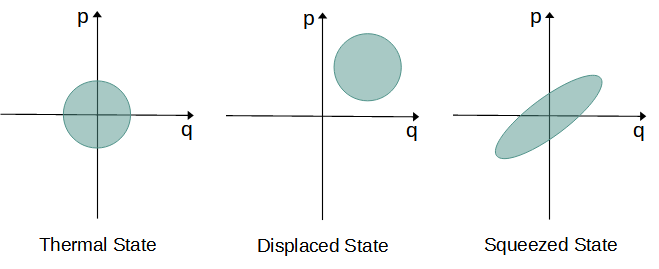
\includegraphics[width=0.6\linewidth]{Images/Gaussian/gaussian-operations.png}
    \caption{Illustration of a single-mode thermal state, displaced coherent state, and squeezed coherent state in the phase space.}
    \label{fig:gaussian-operations}
\end{figure}


\section{Thermal Relaxation of Gaussian States}\label{sec:thermo-gaussian}

% Evolução: equação de lyapunov
% Wigner-Fisher information
As discussed in Chap. \ref{cap:oqs}, the dynamics of an open system can be described by the Lindblad master equation. In our case, we will consider a single bosonic mode (Eq. \eqref{eq:k-harmonic-oscillator} with $k=1$) interacting with a thermal bath and evolving in time according to Davies maps, which has already been calculated in the example in Sec. \ref{sec:example-oscillator},
\begin{equation}
    \frac{d}{dt} {\rho} = -i [{H}, {\rho}] + \Gamma (\bar{n}+1) \mathcal{D}_a({\rho}) + \Gamma \bar{n}\mathcal{D}_{a^\dagger} ({\rho}),
    \label{eq:lindblad-gaussian}
\end{equation}

\noindent where $\Gamma$ is the dissipation rate and $\bar{n} = 1/(e^{\beta \omega} - 1)$ is the Bose distribution. Recalling the jump operators of Eq. \eqref{eq:jump-oscillator}, we can rewrite $\mathcal{D}^-({\rho})= \Gamma (\bar{n}+1) \mathcal{D}_a({\rho})$ and $\mathcal{D}^+({\rho})= \Gamma \bar{n}\mathcal{D}_{a^\dagger} ({\rho})$. Because this is a Davies maps, we know that the final state will always be a thermal state with mean vector $\mathbf{v}_{eq} = 0$ and a covariance matrix equal to $\Theta_{eq} = f(\beta) \mathbb{I}$, where $f(\beta) = \bar{n} + 1/2$.

As elaborated in Sec. \ref{sec:gaussian}, it is convenient to use the phase-space representation instead of the density matrix. For this reason, we will rewrite Eq. \eqref{eq:lindblad-gaussian} in terms of the mean vector and the covariance matrix using that $\frac{d}{dt} \braket{O}_\rho = \text{Tr}[O \frac{d}{dt}\rho]$. The mean vector of a single mode has the form $\mathbf{v}_t = (\braket{{a}}, \braket{{a}^\dagger})^T$. To find its time derivative, we compute
\begin{align}
    &\frac{d}{dt}\braket{{a}} = -\left( i\omega + \frac{\Gamma}{2} \right) \braket{{a}}\\
    &\frac{d}{dt}\braket{{a}^\dagger} = \left( i\omega - \frac{\Gamma}{2} \right) \braket{{a}^\dagger},
\end{align}

\noindent which gives the differential equation 
\begin{equation}
    \dot{\mathbf{v}}_t = \Lambda \mathbf{v}_t,
    \label{eq:dt-mean-vector}
\end{equation}
\noindent where
\begin{equation}
    \Lambda = -\frac{1}{2}
    \begin{bmatrix}
        \Gamma + 2i\omega & 0\\
        0 & \Gamma - 2i\omega
    \end{bmatrix}.
\end{equation}

\noindent The covariance matrix of a single mode is structured as
\begin{equation}
    \Theta_t =
    \begin{bmatrix}
        \frac{1}{2}(\braket{{a}^\dagger {a}} + \braket{{a} {a}^\dagger}) - \braket{{a}^\dagger} \braket{{a}} & \braket{{a}^2} - \braket{{a}}^2\\
        \braket{{a}^{\dagger 2}} - \braket{{a}^\dagger}^2 & \frac{1}{2}(\braket{{a}^\dagger {a}} + \braket{{a} {a}^\dagger}) - \braket{{a}^\dagger} \braket{{a}}
    \end{bmatrix}.
\end{equation}

\noindent To take its time derivative, we first compute
\begin{align}
    &\frac{d}{dt}\braket{{a} {a}^\dagger} = -\Gamma (\braket{{a}{a}^\dagger} - \bar{n} - 1),\\
    &\frac{d}{dt}\braket{{a}^\dagger {a}} = -\Gamma (\braket{{a}{a}^\dagger} - \bar{n}),\\
    &\frac{d}{dt}\braket{{a}^2} = -(2i\omega + \Gamma)\braket{{a}^2},\\
    &\frac{d}{dt}\braket{{a}^{\dagger 2}} = (2i\omega - \Gamma)\braket{{a}^{\dagger 2}},
\end{align}

\noindent to obtain the following differential equation called the Lyapunov Equation,
\begin{equation}
    \dot{\Theta}_t = \Lambda \Theta + \Theta \Lambda^\dagger + F,
    \label{eq:lyapunov}
\end{equation}

\noindent where $F = \Gamma f(\beta) \mathbb{I}$. Therefore, by solving Eqs. \eqref{eq:dt-mean-vector} and \eqref{eq:lyapunov}, we find that the time evolution of a single-mode Gaussian state is given by
\begin{align}
    &\mathbf{v}_t = e^{-\Gamma t} (\braket{a}_0 e^{-i \omega t}, \braket{a^\dagger}_0 e^{i \omega t})^T\\
    &\Theta_t^{11} = \Theta_t^{22} = c_{0} e^{-\Gamma t} + f(\beta),\\
    &\Theta_t^{12} = (\Theta_t^{21})^* = d_{0} e^{-(\Gamma + 2i\omega)t},
\end{align}

\noindent where $c_0$, $d_0$, $\braket{a}_0$, and $\braket{a^\dagger}_0$ are constants obtained from the initial conditions.

To analyse the thermal relaxation of a Gaussian state from a thermodynamic perspective, we will rewrite some information and thermodynamic quantities we defined in Chap. \ref{cap:thermo} in terms of the mean vector and covariance matrix. Because the asymmetry only occurs in the far-from-equilibrium regime, it will be useful to find the nonequilibrium free energy of a Gaussian state. As we did in Sec. \ref{sec:thermo-variables}, we will start with the average energy of a Gaussian state with Wigner distribution $W(\mathbf{x})$, which is defined as
\begin{equation}
    E(W(\mathbf{x})) = \omega \int |\mathbf{x}|^2 W(\mathbf{x}) d^2 \mathbf{x}.
\end{equation}

\noindent Using that the Wigner distribution of an arbitrary thermal state is
\begin{equation}
    W_{th}(\mathbf{x}) = \frac{e^{-|\mathbf{x}|^2 / f(\beta)}}{\pi f(\beta)},
\end{equation}

\noindent we can substitute $|\mathbf{x}|^2 = -f(\beta)(\ln(\pi f(\beta)) + \ln W_{th}(\mathbf{x}))$ in the average energy to obtain
\begin{equation}
    \begin{split}
        E(W(\mathbf{x})) &= -\omega f(\beta) \int W(\mathbf{x}) (\ln(\pi f(\beta)) + \ln W_{th}(\mathbf{x})) d^2 \mathbf{x}\\
        &= -\omega f(\beta) \left[ \ln(\pi f(\beta)) + \int W(\mathbf{x}) \ln W_{th}(\mathbf{x}) d^2 \mathbf{x} \right],
    \end{split}
\end{equation}

\noindent where we used $\int W(\mathbf{x}) d^2 \mathbf{x} = 1$. Similar to what we did in Eq. \ref{eq:energia-krissia}, we will introduce the Wigner entropy defined as
\begin{equation}
    S_W(W(\mathbf{x})) = -\int W(\mathbf{x}) \ln  W(\mathbf{x}) d^2 \mathbf{x} = 1 + \ln \pi + \frac{1}{2} \ln |\Theta|,
    \label{eq:wigner-entropy}
\end{equation}

\noindent and find
\begin{equation}
    \begin{split}
        E(W(\mathbf{x})) &= -\omega f(\beta) \left[ \ln(\pi f(\beta)) + \int W(\mathbf{x}) \ln W_{th}(\mathbf{x}) d^2 \mathbf{x} + S_W(W(\mathbf{x})) - S_W(W(\mathbf{x})) \right]\\
        &= -\omega f(\beta) \left[ \ln(\pi f(\beta)) + \int W(\mathbf{x}) \ln W_{th}(\mathbf{x}) d^2 \mathbf{x} - \int W(\mathbf{x}) \ln  W(\mathbf{x}) d^2 \mathbf{x} - S_W(W(\mathbf{x})) \right]
    \end{split}
\end{equation}

\noindent where we can identify the Wigner relative entropy, that is defined as
\begin{equation}
   \begin{split}
       K[W_1(\mathbf{x}) || W_2(\mathbf{x})] &= \int W_1(\mathbf{x}) \ln \frac{W_{1}(\mathbf{x})}{W_{2}(\mathbf{x})} d^2 \mathbf{x}\\
       &= -1 + \frac{1}{2} \left[(\mathbf{v}_1 - \mathbf{v}_2)^\dagger \Theta_2^{-1} (\mathbf{v}_1 - \mathbf{v}_2) + \text{Tr}(\Theta_2^{-1} \Theta_1) + \ln \frac{|\Theta_2|}{|\Theta_1|} \right].
   \end{split}
   \label{eq:wigner-relative-entropy}
\end{equation}

\noindent As a result, the internal energy of a Gaussian system is
\begin{equation}
    E(W(\mathbf{x})) = \omega f(\beta) K[W(\mathbf{x}) || W_{th}(\mathbf{x})] + \omega f(\beta) S(W(\mathbf{x})) + F_{\text{eq}},
    \label{eq:energy-gaussian}
\end{equation}

\noindent where $F_{\text{eq}} = -\omega f(\beta) \ln (\pi f(\beta))$ is the equilibrium free energy of a thermal state. Given that for Gaussian states the Wigner entropy satisfy conditions analogous to the von Neumann entropy \cite{adesso-2016}, we can extend the Helmholtz free energy to $F(W) = E(W) - \omega f(\beta)S_W(W)$. Using this free energy and considering that $W_{th}(\mathbf{x}) = W_{\text{eq}}(\mathbf{x})$ is the equilibrium state, we can define a nonequilibrium free energy of a Gaussian state as
\begin{equation}
    F_{\text{neq}}(W(\mathbf{x})) = \omega f(\beta) K[W(\mathbf{x}) || W_{\text{eq}}(\mathbf{x})] + F_{\text{eq}},
\end{equation}

\noindent which is similar to Eq. \ref{eq:fneq}. So, the Wigner relative entropy (Eq. \eqref{eq:wigner-relative-entropy}) is an indicator of how far from the equilibrium our system is. For this reason, when studying the asymmetry in Gaussian states, we will also impose that the hot and cold initial states have the same initial Wigner relative entropy.

As discussed in Chap. \ref{cap:thermo}, another approach to study the nonequilibrium regime is using ergotropy defined in Eq. \eqref{eq:ergotropia}. If we substitute \eqref{eq:energy-gaussian} into Eq. \eqref{eq:ergotropia}, we find
\begin{equation}
    \mathcal{E}(W(\mathbf{x})) = \omega f(\beta) (K[W(\mathbf{x}) || W_{th}(\mathbf{x})] - K[W_\pi(\mathbf{x}) || W_{th}(\mathbf{x})]),
    \label{eq:ergotropy-gaussian-full}
\end{equation}

\noindent where $W_\pi(\mathbf{x})$ is the Wigner function of the passive state that has inverse temperature $\beta_\pi$ defined by $f(\beta_\pi) = \sqrt{|\Theta|}$. Because the passive state of a Gaussian state is always thermal, we can assume $W_{th}=W_\pi$ such that ergotropy becomes
\begin{equation}
    \mathcal{E}(W(\mathbf{x})) = \omega f(\beta_\pi) K[W(\mathbf{x}) || W_{\pi}(\mathbf{x})].
    \label{eq:ergotropy-gaussian-passive}
\end{equation}

\noindent From this expression, we find that every squeezed and displaced state have ergotropy meaning they are in the nonequilibrium regime \cite{huber-2016}. Moreover, squeezing operations can also create coherences in the state, so squeezed states can have quantum resources. An interesting result from Ref. \cite{medina-2025} is that squeezed states with higher initial ergotropy relaxate faster than displaced state, what has been named ergotropic Mpemba effect. They also showed that, even when the initial ergotropy is the same, the squeezed state also relaxate faster than the displaced state. These results inspired the
study of how displacement and squeezing may affect the thermal relaxation asymmetry.

However, instead of assuming the arbitrary thermal state is equal to the passive state, we can assume it is the equilibrium state ($W_{th} = W_{\text{eq}}$). Then, we make the time derivative on Eq. \eqref{eq:ergotropy-gaussian-full} and find that the entropy production for Gaussian states are
\begin{equation}
    \begin{split}
        \Pi_W &= - \frac{d}{dt} K[W(\mathbf{x}) || W_{th}(\mathbf{x})] \\
        &= -\frac{d}{dt} K[W_\pi(\mathbf{x}) || W_{th}(\mathbf{x})] - \frac{\dot{\mathcal{E}}}{\omega f(\beta)}\\
        &= \Pi_\pi - \frac{\dot{\mathcal{E}}}{\omega f(\beta)},
    \end{split}
    \label{eq:sprod-passive-ergotropic-gaussian}
\end{equation}

\noindent which is similar to Eq. \eqref{eq:sprod-passive-ergotropic}. So it is also possible to separate the entropy production of Gaussian states into a passive and an ergotropic contribution.

Now that we briefly redefined some thermodynamic quantities for Gaussian states, we will discuss how the thermal kinematics change in this regime. As discussed in Sec. \ref{sec:thermal-kinematics}, Fisher information is the essential quantity for the thermal kinematics approach of heating-cooling asymmetry. To find a Fisher information for Gaussian states, we will follow the same procedure of Sec. \ref{sec:thermal-kinematics} and make a second order Taylor expansion in a parameter $\theta$ of the Wigner relative entropy (Eq. \eqref{eq:wigner-relative-entropy}) as
\begin{equation}
    \begin{split}
        K[W(\mathbf{x}, \theta+d\theta) || P(\mathbf{x}, \theta)] &= \int W(\mathbf{x}, \theta+d\theta) \ln \left ( \frac{W(\mathbf{x}, \theta+d\theta)}{W(\mathbf{x}, \theta)} \right ) d^2 \mathbf{x} \\
        &= \int [W(\mathbf{x}, \theta) + \partial_\theta W(\mathbf{x}, \theta) d\theta + \frac{1}{2} \partial_\theta^2 W(\mathbf{x}, \theta) d\theta^2 + \mathcal{O}(d\theta^3)] \times\\
        &\times \left[\frac{\partial_\theta W(\mathbf{x}, \theta)}{W(\mathbf{x}, \theta)} d\theta + \frac{1}{2}\frac{\partial_\theta^2 W(\mathbf{x}, \theta)}{W(\mathbf{x}, \theta)} d\theta^2 + \mathcal{O}(d\theta^3) \right] d^2 \mathbf{x} \\
        &= \int \frac{(\partial_\theta W(\mathbf{x}, \theta) d\theta)^2}{W(\mathbf{x}, \theta)} d^2 \mathbf{x} + \mathcal{O}(d\theta^3)\\
        &= \frac{1}{2} \mathcal{I}_W(\theta) d\theta^2 + \mathcal{O}(d\theta^3),
    \end{split}
\end{equation}

\noindent where we identify $\mathcal{I}_W(\theta)$ as the Wigner-Fisher information, that can be written in terms of the mean vector and the covariance matrix resulting in
\begin{equation}
    \mathcal{I}_W (t) = \dot{\mathbf{v}}_t^\dagger \Theta^{-1}_t \dot{\mathbf{v}}_t + \text{Tr}[(\Theta_t^{-1} \dot{\Theta}_t)^2].
    \label{eq:wigner-fisher}
\end{equation}

\noindent Note that we changed $\theta=t$ because in thermal kinematics the interesting parameter is time, and, as a result, the thermal kinematics variables become 
\begin{align}
    &v_W(t) =  \sqrt{\frac{1}{2}\mathcal{I}_W ({\rho}(t))} \label{eq:velocidade-gaussian}\\
    &\mathcal{L}_W(t) = \int_0^{t} \sqrt{\frac{1}{2}\mathcal{I}_W ({\rho}(t))} \label{eq:comprimento-gaussian}\\
    &\varphi_W(t_s) = \frac{\mathcal{L}_W(t_s)}{\mathcal{L}_W(t_f)}. \label{eq:completion-gaussian}
\end{align}

\noindent Additionally, the Wigner-Fisher information can be separated into a passive and ergotropic contribution: $\mathcal{I}_W (t) = \mathcal{I}_\pi (t) + \mathcal{I}_\mathcal{E} (t)$. To see this, we will use that the passive state of any Gaussian state is always thermal, so the first term of Eq. \eqref{eq:wigner-fisher} is zero because $\mathbf{v}_\pi = 0$. Then, using that the covariance matrix is $\Theta_\pi = f(\beta_\pi) \mathbb{I}$ where $f(\beta_\pi) = \sqrt{|\Theta|}$, we find $\Theta_\pi^{-1} = (1/f(\beta_\pi))\mathbb{I}$ and $\dot{\Theta}_\pi = f(\beta_\pi) \dot{S}_W(t) \mathbb{I}$. Substituting these matrices in the second term of Eq. \eqref{eq:wigner-fisher}, we obtain the passive contribution in the Wigner-Fisher information is
\begin{equation}
    \begin{split}
        \mathcal{I}_\pi (t) &= \text{Tr}[(\Theta_t^{-1} \dot{\Theta}_t)^2]\\
        &= \text{Tr}\left[\left(\frac{1}{f(\beta_\pi)} f(\beta_\pi) \dot{S}_W(t) \mathbb{I}\right)^2\right]\\
        &= 2 \dot{S}_W^2 (t)
    \end{split}
\end{equation}

With this, we introduced all the necessary quantities and can start discussing our results. First, we will discuss the heating-cooling asymmetry for thermal states in Sec. \ref{sec:result-thermal}. Then we will investigate the consequences of displacing this thermal state in Sec. \ref{sec:result-displaced} and squeezing this thermal state in Sec. \ref{sec:result-squeezed}. Because a squeezed state relaxate faster than a displaced state, we will try to invert the asymmetry by combining these Gaussian operations in Sec. \ref{sec:result-invertion}.

\section{Asymmetry for Thermal States}\label{sec:result-thermal}

In this section, we consider a Gaussian state initially in a thermal state with inverse temperature $\beta_i$ interacting with a bath at inverse temperature $\beta_f$. After solving Eq. \eqref{eq:dt-mean-vector} and Eq. \eqref{eq:lyapunov}, we find the dynamics is described by a zero mean vector ($\mathbf{v}_{th} = 0$) and a covariance matrix equal to $\Theta_{th} = \Delta_\beta \mathbb{I}$, being $\Delta_{\beta} = [f(\beta_i) - f(\beta_f)]e^{-\Gamma t} + f(\beta_f)$ where $\Gamma$ is the dissipation rate, and $f(\beta) = \bar{n} + 1/2$.

Similar to the qubits case, to find two thermodynamically equivalent initial states, we use the Wigner relative entropy defined in Eq. \eqref{eq:wigner-relative-entropy}. Using that for thermal states $|\Theta| = (\Delta_\beta)^2$ and $\Theta^{-1}_{th} = \frac{1}{\Delta_\beta} \mathbb{I}$, being the equilibrium $\lim_{t\rightarrow\infty} \Delta_\beta = f(\beta_f)$, the analytical expression for the Wigner-Fisher information (defined in Eq. \eqref{eq:wigner-fisher}) is
\begin{equation}
    \mathcal{I}_{W_{th}} (t) = 2 \left[ \frac{\partial}{\partial t} \ln \Delta_\beta \right]^2,
\end{equation}

\noindent the statistical velocity (defined in Eq. \eqref{eq:velocidade-gaussian})
\begin{equation}
    v_{W_{th}}(t) = \frac{\partial}{\partial t} \ln \Delta_\beta,
\end{equation}

\noindent and the statistical length (defined in Eq. \eqref{eq:comprimento-gaussian})
\begin{equation}
     \mathcal{L}_{W_{th}} (t) = \ln \left( \frac{[f(\beta_i) - f(\beta_f)]e^{-\Gamma t} + f(\beta_f)}{f(\beta_i)} \right).
     \label{eq:L-termico}
\end{equation}

\noindent The statistical length in the equilibrium is

\begin{equation}
    \mathcal{L}_{W_{th}}^{eq} \equiv \lim_{t \rightarrow \infty} \mathcal{L}_{W_{th}} (t) = \ln\left[ \frac{f(\beta_f)}{f(\beta_i)} \right].
    \label{eq:L-termico-eq}
\end{equation}

\noindent Because of the explicit dependence on $\beta_i$, two states with different initial temperatures that relaxate to the same final temperature will have different statistical lengths. To simplify the notation, we define $f_i \equiv f(\beta_f)/f(\beta_i)$ and $k = \exp(-\Gamma t)$ and use the expressions \eqref{eq:L-termico} and \eqref{eq:L-termico-eq} to write the degree of completion (defined in Eq. \eqref{eq:completion-gaussian}) as
\begin{equation}
    \varphi_{W_{th}}(t) = \frac{\ln (k + (1-k)f_i)}{\ln(f_i)} \equiv \varphi_{i}(k).
    \label{eq:completion-thermal}
\end{equation}

Now, we can analyse the thermal relaxation asymmetry for thermal states. We know that $\beta_c > \beta_f > \beta_h$, which results in $f(\beta_c) < f(\beta_f) < f(\beta_h)$, leading to 
\begin{align}
    &1 > \frac{f(\beta_f)}{f(\beta_h)} = f_h \label{ineq:fbeta-cooling}\\
    &1 < \frac{f(\beta_f)}{f(\beta_c)} = f_c, \label{ineq:fbeta-heating}
\end{align}

\noindent which is equivalent to $\ln(f_c) > 0$ and $\ln(f_h) < 0$. Next, we will use the Jensen inequality for $f(x) = \ln(x)$, that is $f(k x_1 + (1 - k) x_2) \geq kf(x_1) + (1-k) f(x_2)$. In our case, we can use $x_1 = 1$ and $x_2 = f_i$ to obtain
\begin{equation}
    \ln(k + (1 - k) f_i) \geq (1-k) \ln(f_i),
    \label{eq:jensen}
\end{equation}

\noindent where we have the numerator of the degree of completion on the left side and the denominator on the right side. For the heating case ($i=c$), $\ln(f_c) > 0$ so dividing Eq. \eqref{eq:jensen} by it do not change the inequality and we find that the degree of completion (Eq. \eqref{eq:completion-thermal}) for this process is
\begin{equation}
    \varphi_{c} = \frac{\ln (k + (1-k)f_c)}{\ln(f_c)} \geq 1-k.
\end{equation}

\noindent On the other hand, for the cooling case ($i=h$), $\ln(f_h) < 0$ so the division invert the inequality in Eq. \eqref{eq:jensen} and we find that the degree of completion for this process is
\begin{equation}
    \varphi_h = \frac{\ln (k + (1-k)f_h)}{\ln(f_h)} \leq 1-k.
\end{equation}

\noindent By combining both degrees of completion inequalities, we obtain that $\varphi_c \geq \varphi_h$, which means that heating is always faster or equal to cooling a Gaussian thermal state.

\begin{figure}[t]
    \centering
    
\includegraphics[width=0.6\linewidth]{Images/Gaussian/Sprod-thermal.png}
    \caption{Entropy production rate for heating (red) and cooling (blue) thermal states.}
    \label{fig:sprod-thermal}
\end{figure}

It is relevant to study whether the presence of thermal relaxation asymmetry in Gaussian systems is also explained by the difference in entropy production rate. The Wigner relative entropy for a thermal state is
\begin{equation}
    K[W_{th} || W_f] = -1 + \frac{\Delta_\beta}{f(\beta_f)} + \ln \frac{f(\beta_f)}{\Delta_\beta}.
    \label{eq:K-thermal}
\end{equation}

\noindent By taking the negative time derivative of Wigner relative entropy, we find that the entropy production rate is
\begin{equation}
    \Pi_{W_{th}} = \frac{\dot{\Delta}_\beta}{\Delta_\beta} - \frac{\dot{\Delta}_\beta}{f(\beta_f)} = \dot{S}_{W_{th}} \left( 1- \frac{\Delta_\beta}{f(\beta)} \right),
    \label{eq:sprod-thermal}
\end{equation}

\noindent where $\dot{S}_{W_{th}} = \dot{\Delta}_\beta/\Delta_\beta $ is the time derivative of the Wigner entropy (Eq. \eqref{eq:wigner-entropy}). From this expression, we obtain Fig. \ref{fig:sprod-thermal} by using $K[W_c || W_f] = K[W_h || W_f] = 0.5$ and $T_f = 2$ (in natural units). Note that heating entropy production reaches zero before cooling, corroborating our conclusion that heating relaxes faster than cooling. Also, heating has an initially higher entropy production rate than cooling, which explains the asymmetry.





\section{Asymmetry for Displaced States}\label{sec:result-displaced}

Now, we can analyse what happens to the asymmetry when we displace a thermal state. The solution of Eq. \eqref{eq:dt-mean-vector} and Eq. \eqref{eq:lyapunov} is that the mean vector becomes $\vec{v}_d = (\mu_t, \mu_t^*)$ where $\mu_t = \mu e^{-(i\omega + \Gamma / 2)t}$ while the covariance matrix remains unchanged, i.e., $\Theta_d = \Delta_\beta \mathbb{I}$. Using these results in the Wigner relative entropy (Eq. \eqref{eq:wigner-relative-entropy}), we find
\begin{equation}
    K[W_d || W_f] = -1 + \frac{|\mu|^2}{f(\beta_f)} e^{-\Gamma t} + \frac{\Delta_\beta}{f(\beta_f)} + \ln \frac{f(\beta_f)}{\Delta_\beta}.
    \label{eq:K-displaced}
\end{equation}

\noindent The term containing the displacement parameter ($\mu$) is independent of the system's initial temperature, which means that, regardless of the initial temperature, applying a displacement operator to any thermal state results in the same shift in their Wigner relative entropy. Thus, for simplicity, we chose two equidistant thermal states and then applied the same amount of work on both (which is equivalent to using the same $\mu$). However, because displacement also adds ergotropy to the state, it is important to use initial states with the same ergotropy. The ergotropy for a displaced state is $\mathcal{E}_d= |\mu|^2 e^{-\Gamma t}$, which means that using the same $\mu$ is enough to guarantee different states have the same ergotropy. As we did before, we could try to analytically calculate the thermal kinematics variables, but the Wigner-Fisher information for a displaced state is
\begin{equation}
    I_{W_d} (t) = \frac{2}{\Delta_\beta} \left[ \frac{\dot{\Delta}_\beta^2}{\Delta_\beta} + \left(\omega^2 + \frac{\Gamma^2}{4} \right)|\mu|^2 e^{-\Gamma t} \right],
    \label{eq:WFI-displaced}
\end{equation}

\begin{figure}[t]
    \centering
    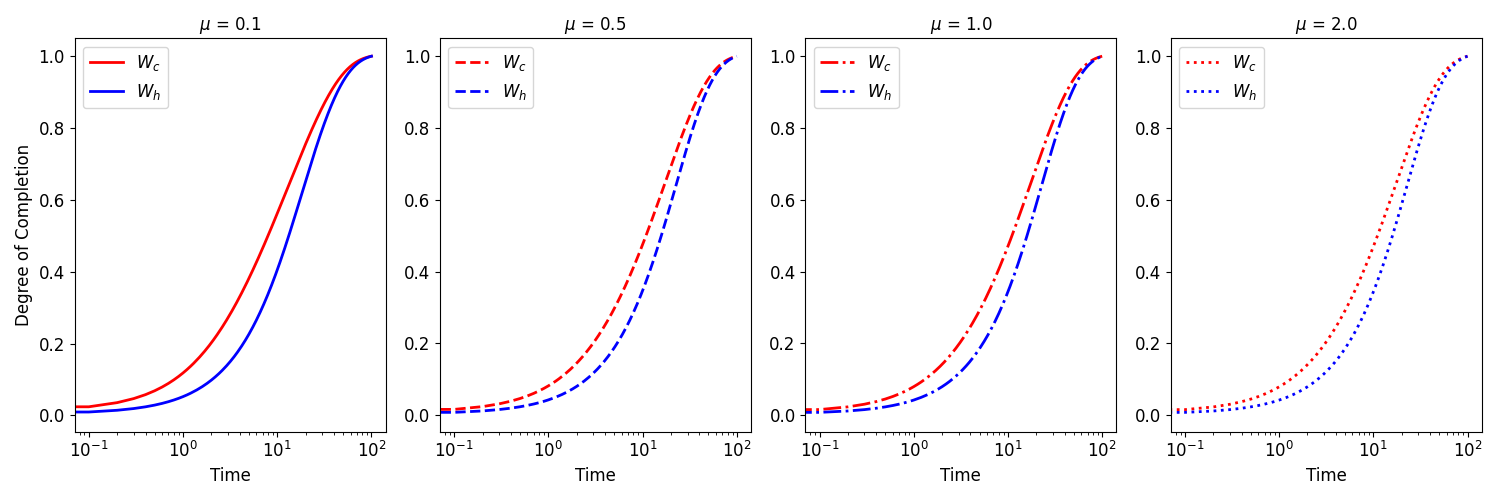
\includegraphics[width=\linewidth]{Images/Gaussian/completion-displaced.png}
    \caption{Degree of completion for a displaced thermal state. Each graph corresponds to a different displacement parameter ($\mu$).}
    \label{fig:completion-displaced}
\end{figure}

\begin{figure}[b!]
    \centering
    
\includegraphics[width=0.7\linewidth]{Images/Gaussian/Vw-displaced.png}
    \caption{Statistical velocity of a displaced thermal state as a function of time. Each curve corresponds to a different displacement parameter ($\mu$).}
    \label{fig:velocity-displaced}
\end{figure}

\noindent and, despite being possible to analytically find the statistical velocity and length, the complexity of the final expressions ultimately makes it difficult to extract useful information. Therefore, we use a numerical approach for this case. The chosen parameter were $\omega = 1$, $\Gamma = 0.1$, $T_f = 2$, and $K[W_c || W_f] = K[W_h || W_f] = 0.5$. Fig. \ref{fig:completion-displaced} shows the degree of completion for different displacement parameters, with the thermal relaxation of $W_c$ (in red) being faster than that of $W_h$ (in blue) for all the displacements. An interesting result is that increasing the displacement parameter, moves the initial state further away from the equilibrium (as one can see from Eq. \eqref{eq:K-displaced}), but the heating-cooling asymmetry remains unchanged. However, the initial statistical velocity also increase with $\mu$ as shown in Fig. \ref{fig:velocity-displaced} and expected from Eq. \eqref{eq:WFI-displaced}. Therefore, a possible explanation for the asymmetry remaining unchanged with displacement is that the initial distance from equilibrium is compensated by a higher initial velocity.

\begin{figure}[t]
    \centering
    
\includegraphics[width=\linewidth]{Images/Gaussian/Sprod_contributions_displaced.png}
    \caption{Total entropy production rate(solid) with its ergotropic (dotted) and passive (dashed) contributions for heating (red) and cooling (blue) equidistant displaced thermal states.}
    \label{fig:sprod-displaced-contributions}
\end{figure}


Another way to analyse this asymmetry is using the entropy production. Given that displacement generates ergotropy in the system, we can use the entropy production separation into passive and ergotropic contribution from Eq. \eqref{eq:sprod-passive-ergotropic-gaussian}. The total entropy production rate for a displaced state is given by
\begin{equation}
    \Pi_{W_d} = \frac{1}{f(\beta)} (\Gamma |\mu|^2 e^{-\Gamma t} - \dot{\Delta}_\beta) + \frac{\dot{\Delta}_\beta}{\Delta_\beta}.
    \label{eq:sprod-displaced}
\end{equation}

\noindent The entropy production of the passive state is
\begin{equation}
    \Pi_{W_\pi} = \dot{S}_{W_\pi} \left( 1- \frac{f(\beta_\pi)}{f(\beta)} \right) = \Pi_{W_{th}},
    \label{eq:passive-displaced-contribution}
\end{equation}

\noindent which is the same entropy production of the thermal state (Eq. \eqref{eq:sprod-thermal}), because displacement do not change the covariance matrix, resulting in $f(\beta_\pi) = \Delta_\beta$ and $\dot{S}_{W_{\pi}} = \dot{S}_{W_{th}}$. Finally, the ergotropic contribution is in terms of the ergotropic loss rate: $\dot{\mathcal{E}}_d= -\Gamma|\mu|^2 e^{-\Gamma t}$. Fig. \ref{fig:sprod-displaced-contributions} shows the total entropy production rate (solid line), its passive contribution (dashed line) and ergotropic contribution (dotted line). Each plot has an increasing displacement parameter $\mu$ from left to right, being $W_c$ in red and $W_h$ in blue. In all the graphs, $W_c$ starts with a higher total entropy production rate than $W_h$, which again explains why the thermal relaxation of $W_c$ is faster. In addition, making greater displacements increases the ergotropic contribution while keeping the passive contribution unchanged. As a consequence, the total entropy production increases with $\mu$ because of the ergotropic contribution. Another interesting result is that, when comparing $W_c$ and $W_h$ with same $\mu$, the ergotropic contribution do not change, meaning the passive contribution is the generator of asymmetry that is unaffected by the displacement operation, which agrees with our previous discussion.






\section{Asymmetry for Squeezed States}\label{sec:result-squeezed}

In this section, we study the thermal relaxation asymmetry of squeezed thermal states. Unlike the displacement operation, squeezing a thermal state preserves the zero mean vector and changes the covariance matrix to
\begin{equation}
    \Theta_s = f(\beta_t) 
    \begin{bmatrix}
        \cosh(2 r_t) & -e^{i \phi_t} \sinh(2r_t)\\
        -e^{-i \phi_t} \sinh(2r_t) & \cosh(2 r_t)
    \end{bmatrix},
\end{equation}

\noindent where $\phi_t$ is the squeezing phase, the squeezing parameter is implicitly defined as
\begin{equation}
    \cosh(2r_t) = \frac{1}{f(\beta_t)} [\Delta_\beta + 2f(\beta_i) e^{-\Gamma t} \sinh^2(r)],
    \label{eq:coshrt-squeezing}
\end{equation}

\noindent and $\beta_t$ is implicitly defined by
\begin{equation}
    f(\beta_t) = \sqrt{\Delta_\beta^2 + 4 f(\beta_i) f(\beta) e^{-2\Gamma t} (e^{\Gamma t} - 1) \sinh^2(r)}.
    \label{eq:fbetat-squeezing}
\end{equation}

\noindent With the information above, the relative entropy for a squeezed state is
\begin{equation}
    K[W_s || W_f] = -1 + \frac{f(\beta_t)}{f(\beta)}\cosh(2r_t) + \ln \left( \frac{f(\beta)}{f(\beta_t)} \right).
    \label{eq:relative-entropy-squeezing}
\end{equation}

\noindent Different from the displacement case, because the $r_t$ and $f(\beta_t)$ that contains the initial temperature are related, doing the same squeezing in different thermal states do not preserve their equidistance. As a consequence, to make a fair comparison, we must use different squeezing parameters for each state. Just like displacement, squeezing also generates ergotropy in the state, so it is important to choose initial states with same ergotropy. The ergotropy of a squeezed thermal state is
\begin{equation}
    \mathcal{E}_s(t) = \omega f(\beta_t) (\cosh (2r_t) - 1).
    \label{eq:ergo-squeezing}
\end{equation}

\noindent Because of the dependence of $f(\beta_t)$, in $t=0$, $f(\beta_t) = f(\beta_i)$ and applying the same squeezing (that is, the same $r$ and $\phi$) in different thermal states results in a higher ergotropy to the squeezed hotter state. For clarity, we will describe how we choose a state with same initial relative entropy and ergotropy. To start, we choose an initial relative entropy $K_0$ and a squeezing parameter for the hotter state ($r_h$), for example. Then, we look for the temperature $T_h$ a thermal state must have to satisfy $K[W_h || W_f] = K_0$ after squeezing with parameter $r_h$. After finding our hotter initial state, we can try to find the colder initial state. By combining Eq. \eqref{eq:relative-entropy-squeezing} and Eq. \eqref{eq:ergo-squeezing}, we get that $f(\beta_c) - f(\beta_h) + f(\beta_f)\ln(f(\beta_h)/f(\beta_c))=0$ must be true to satisfy the condition of same initial relative entropy and ergotropy. Given that we already know $T_h$, we can solve this equation to obtain the temperature of the cold squeezed state and use Eq. \eqref{eq:coshrt-squeezing} to find $r_c$. We will call the initial hotter state $W_h$ and the initial colder state $W_c$. Squeezed states do not have a real temperature, but because the passive state is always a thermal state, we will assume that $W_h$ will cool down and $W_c$ will heat up. Fig. \ref{fig:initial-squeezing} presents Wigner relative entropy as a function of temperature and shows which initial temperatures we find in the end of this process. The left plot corresponds to the smaller squeezing parameters and the right plot corresponds to the bigger squeezing parameters. Note that increasing the squeezing parameter almost conserves de difference between $r_c$ and $r_h$. However, the colder temperature (in blue) have a bigger variation than the hotter temperature (in red), resulting in a bigger variation of ergotropy. From this, it seems that colder states are more sensible to variations on the squeezing parameter.

\begin{figure}[t]
    \centering
    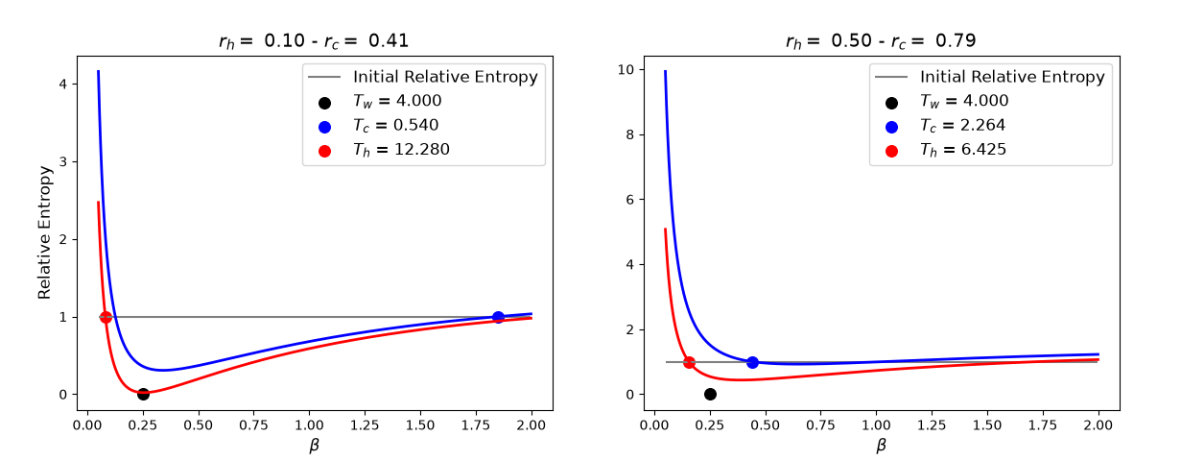
\includegraphics[width=\linewidth]{Images/Gaussian/initialization-squeezing.png}
    \caption{Wigner relative entropy of a squeezed thermal state and the equilibrium thermal state as a function of inverse temperature. The black line indicates the chosen initial Wigner relative entropy that both hot (red dot) and cold (blue dot) squeezed states must have. The left plot uses a small squeezing parameters and the right plot use bigger squeezing parameters.}
    \label{fig:initial-squeezing}
\end{figure}

The Wigner-Fisher information of a squeezed thermal state is
\begin{equation}
    I_{W_s} (t) = 2 \dot{S}_{W_s}^2 + 8 \dot{r}_t^2 + 2 \dot{\phi}_t^2 \sinh^2 (2r_t),
    \label{eq:Iw-squeezing}
\end{equation}

\noindent where the time derivative of the Wigner entropy is
\begin{equation}
    \dot{S}_{W_s} = \frac{\dot{f}(\beta_t)}{f(\beta_t)}.
    \label{eq:Sw-squeezing}
\end{equation}

\begin{figure}[t]
    \centering
    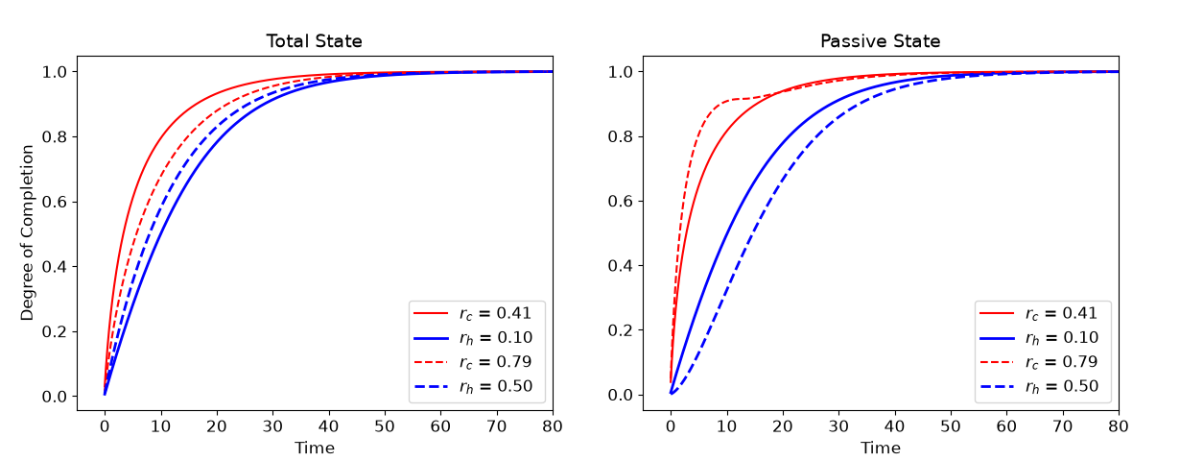
\includegraphics[width=\linewidth]{Images/Gaussian/completion-squeezing.png}
    \caption{Degree of completion for squeezed thermal states (left) and their passive states (right). We compared a smaller squeezing parameter (solid lines) with a bigger squeezing parameter (dashed lines) for both initially colder ($r_c$) and hotter ($r_h$) states.}
    \label{fig:completion-squeezing}
\end{figure}

\noindent Again, obtaining the analytical thermal kinematic expressions from Eq. \eqref{eq:Iw-squeezing} will not bring additional information, so we will solve it numerically. In Fig. \ref{fig:completion-squeezing}, we show the degree of completion as a function of time for the squeezed thermal state (left) and its passive state (right). In each plot, we compared a squeezing with small parameters (solid lines) with a squeezing with bigger parameters (dashed lines). In the both plots, because $W_c$ (in red) is always above $W_h$ (in blue), we can say that heating is faster than cooling for these squeezed states and their passive states. However, in the left plot, by comparing the solid lines with the dashed lines, we observe that increasing the squeezing parameters reduces the heating-cooling asymmetry of the total state. However, in the right plot, the asymmetry in the passive states seems to increase as we increase the squeezing parameters.

To investigate this behaviour, we will analyse the entropy production rate and separate into its passive and ergotropic contribution from Eq. \eqref{eq:sprod-passive-ergotropic-gaussian}. The total entropy production rate is
\begin{equation}
    \Pi_{W_s} = \dot{S}_{W_s} - \frac{\dot{E}}{\omega f(\beta_f)},
\end{equation}

\noindent where the time derivative of the Wigner entropy was calculated in Eq. \eqref{eq:Sw-squeezing} and the last term is the time derivative of the energy,
\begin{equation}
    \dot{E} = \omega[\dot{f}(\beta_t) \cosh (2r_t) + 2 \dot{r}_t f(\beta_t) \sinh(2r_t)].
\end{equation}

\noindent The passive state have $f(\beta_\pi) = f(\beta_t)$, resulting in the entropy production
\begin{equation}
    \Pi_{W_\pi} = \dot{S}_{W_s} \left( 1- \frac{f(\beta_t)}{f(\beta_f)} \right),
\end{equation}

\noindent which depends on the squeezing parameter, so it will change for all of our curves. According to Eq. \eqref{eq:sprod-passive-ergotropic-gaussian}, to find the ergotropic contribution, we take the time derivative of Eq. \eqref{eq:ergo-squeezing} and find
\begin{equation}
    \frac{\dot{\mathcal{E}}_s}{\omega f(\beta_f)} = \frac{\dot{f}(\beta_t)}{f(\beta_f)}(\cosh(2r_t) - 1 ) + 2\frac{{f}(\beta_t)}{f(\beta_t)} \sinh(2r_t)\dot{r}_t.
\end{equation}

\noindent As this equation depends on the squeezing parameter and initial temperature, we find out the ergotropic contribution will also change for all of our curves.

\begin{figure}[b!]
    \centering
    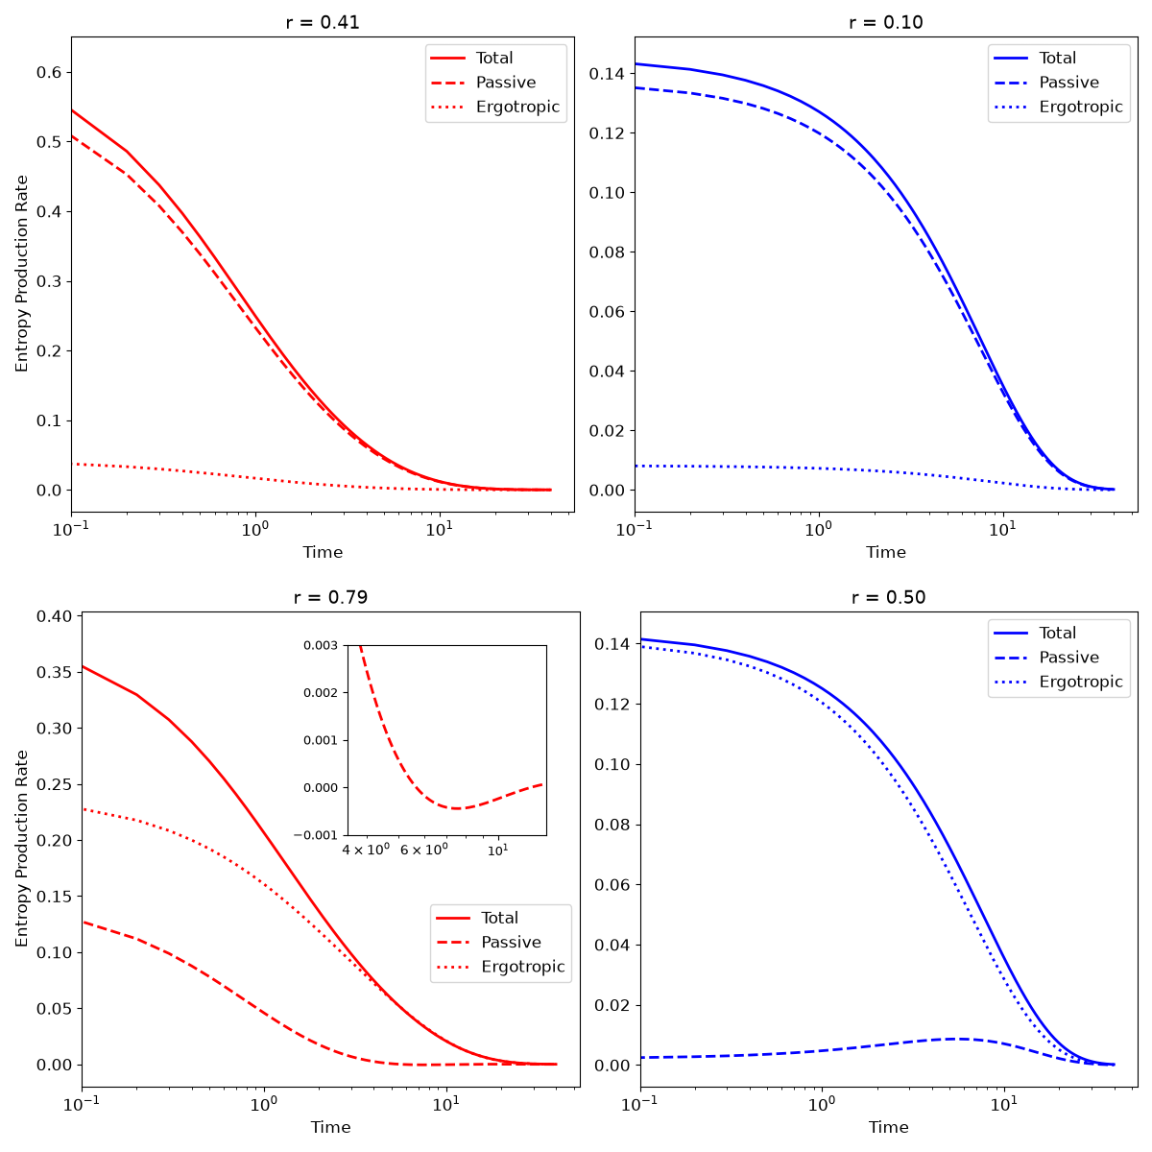
\includegraphics[width=0.8\linewidth]{Images/Gaussian/Sprod-contribution-squeezing.png}
    \caption{Entropy production rate for heating (red) and cooling (blue) squeezed thermal states with smaller parameters (upper plots) and bigger parameters (lower plots). We separate the passive contribution (dashed) and ergotropic contribution (dotted) of the total entropy production rate (solid). The inset plot show the region where the passive state entropy production becomes negative.}
    \label{fig:contribution-squeezing}
\end{figure}

Fig. \ref{fig:contribution-squeezing} show the entropy production rate, where the upper plots correspond to smaller $r$ and the lower plots correspond to bigger $r$. Each graph shows the total entropy production rate (solid line) with its passive (dashed line) and ergotropic (dotted line) contributions. First, the initial total entropy production of $W_c$ is bigger than the initial total entropy production of $W_h$, which explain why heating is faster than cooling again. Also, when we increase the squeezing parameters, the heating and the cooling total entropy productions decrease, but the heating process suffers a bigger reduction when compared with cooling. This can be explained by the previous discussion that colder states have higher sensibility to squeezing variations. As a result, for bigger squeezing parameters, the difference in initial total entropy production between heating and cooling is smaller, which explains why the asymmetry was reduced for the total squeezed state. However, as we already noticed in the equations of entropy production, unlike the displacement operation, squeezing affects both passive and ergotropic contributions, which means that the asymmetry is not fully generated by the passive state. When we look at the passive contribution, the difference between the initial entropy production of heating and cooling becomes bigger as we increase the squeezing parameter. This can explain why the asymmetry in the passive contribution increases. The explanation of how these related quantities can have opposite behaviours with the increase of squeezing parameter is in the ergotropic contribution. Given that for small $r$ the passive contribution was bigger, to preserve the same entropy production, the ergotropic contribution should compensate the decrease of the passive. However, this is not the case and ergotropic increase do not compensate the passive loss as shown in Fig. \ref{fig:contribution-squeezing}.


One last comment of this section is regarding the oscillation in the degree of completion that appears for the passive state of the big squeezing parameter case (red dashed line of the right plot in Fig. \ref{fig:completion-squeezing}). Additionally, the statistical velocity of this same passive state is shown in Fig. \ref{fig:velocity-squeezing-passive} and also presents this oscillation. Recalling the degree of completion and statistical velocity we had for the interacting qubits, we also saw this oscillations and attributed them to a local non-Markovian dynamics witnessed as negative entropy production. The inset in Fig. \ref{fig:contribution-squeezing} shows that the entropy production of the passive state with big squeezing parameter also have negative value for a period of time, which is a signature of non-Markovianity. From this observations, we can again affirm that non-Markovianity may be related to faster relaxation. The origin of this non-Markovian dynamics for the passive state can be understood as a part of squeezing being converted into energy for the passive state. It is interesting that this behaviour was only observed for heating state with big squeezing parameter and not in the correspondent cooling state. One possibility is that the squeezing parameter used in heating was bigger than the one in cooling. However, this cooling process do have a different behaviour, which is a small increase in its entropy production and statistical velocity. This means that, instead of receiving a feedback information from the environment, the system accelerates and loose more information to the environment. We do not know its cause, but it is important to highlight that, while negative entropy production indicate non-Markovianity, the opposite is not always true, i.e., non-Markovian dynamics without negative entropy production is possible \cite{popovic-2018}.

\begin{figure}[t]
    \centering
    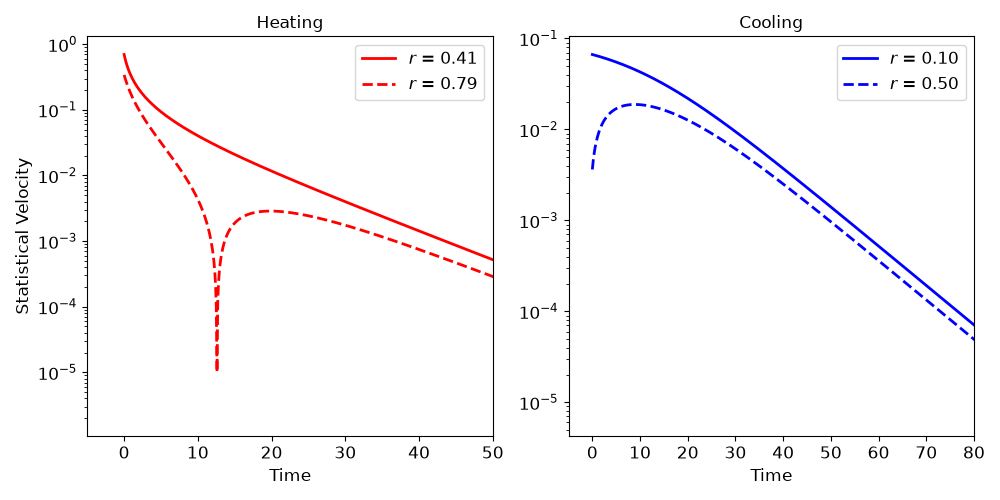
\includegraphics[width=0.8\linewidth]{Images/Gaussian/Vw-squeezing-passive.png}
    \caption{Statistical velocity of the heating (red) and cooling (blue) passive states of squeezed states with smaller parameter (solid lines) and bigger parameters (dashed lines).}
    \label{fig:velocity-squeezing-passive}
\end{figure}



\section{Asymmetry Inversion for Gaussian States}\label{sec:result-invertion}

Until this moment, we only observed that heating was faster than cooling, but previous works have shown that this is not always true \cite{vu-2021, bravetti-2025, teza-2026}. In this section, we will try to invert this asymmetry using the previous observation that squeezed states relaxate faster than displaced states. So, we will apply a squeezing operation on the slower process, that is cooling, and will apply a displacement operation on heating because both initial state must have the same initial ergotropy.

To find a hotter squeezed state and colder displaced state with the same initial relative entropy and ergotropy, we will use a similar approach as the one from Sec. \ref{sec:result-squeezed}. We combine $K[W_s || W_f] = K[W_d || W_f]$ and $\mathcal{E}_s = \mathcal{E}_d$ to obtain $f(\beta_d) - f(\beta_s) + f(\beta_f)\ln(f(\beta_s)/f(\beta_d))=0$, which can be used to find the temperature of a state from the the other state.

\begin{figure}[t]
    \centering
    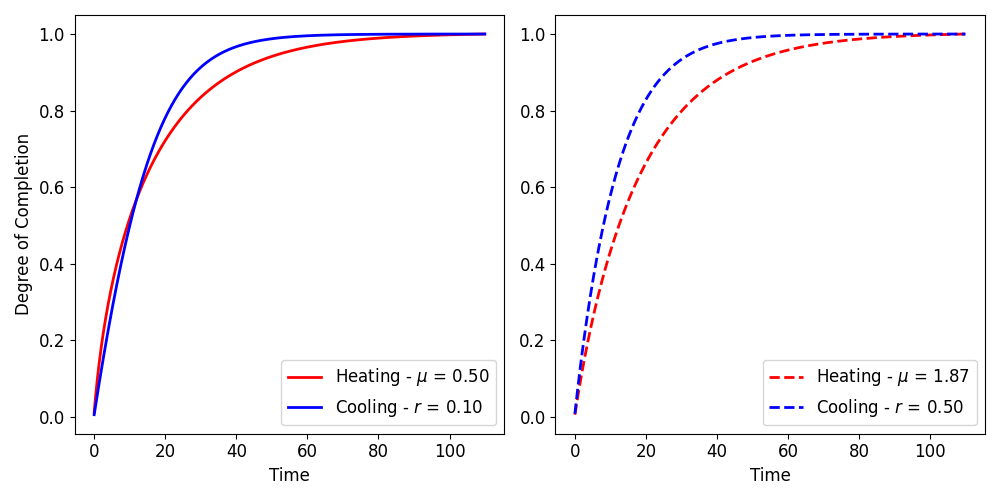
\includegraphics[width=0.8\linewidth]{Images/Gaussian/completion-invertion.png}
    \caption{Degree of completion for heating the displaced state (red) and cooling the squeezed state (blue).}
    \label{fig:completion-inversion}
\end{figure}

The degree of completion for this system is presented in Fig. \ref{fig:completion-inversion}, and shows that it is possible to invert the asymmetry depending on the initial state condition. In the left graph, the displacement and squeezing parameters are smaller than in the right graph, and the asymmetry inversion is partial because cooling is faster only after some time. In the right graph, where the parameters are bigger, cooling is faster than heating for all times. Fig. \ref{fig:completion-inversion-passive} show the degree of completion of the passive states. Despite the inversion of the total state, the passive states still have heating faster than cooling as expected from the thermal states results in Sec. \ref{sec:result-thermal}. Also, we notice that increasing the ergotropy of the total state, makes the passive relaxation slower, but it seems to preserve the asymmetry between heating and cooling.

\begin{figure}[b!]
    \centering
    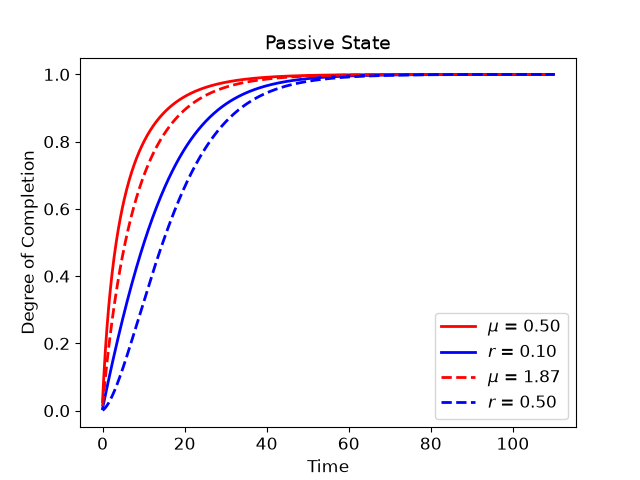
\includegraphics[width=0.5\linewidth]{Images/Gaussian/completion-invertion-passive.png}
    \caption{Degree of completion of the passive state of the heating displaced state (red) and of the cooling squeezed state (blue).}
    \label{fig:completion-inversion-passive}
\end{figure}

To study the entropy production rate of heating the displaced state, we used the same expressions of Section \ref{sec:result-displaced} and, for the entropy production rate of cooling the squeezed state, we used the expressions of Section \ref{sec:result-squeezed}. Fig. \ref{fig:sprod-inversion} shows the total entropy production (solid lines), the passive (dashed lines) and the ergotropic (dotted lines) contributions for the entropy production of smaller and bigger parameters, respectively. Given that heating is faster for the passive states, what accelerates cooling to create the inversion must be the ergotropic contribution. Different from the results comparing only squeezing or only displacement, the ergotropic contribution of cooling (squeezing) is initially higher than the one of heating, which explains the full inversion of the asymmetry. Furthermore, for the partial inversion, we see that the ergotropic part had almost no participation in the relaxation and all the asymmetry was generated by the passive state. In this case, heating had higher initial entropy production and was faster than cooling according to the degree of completion in Fig. \ref{fig:completion-inversion}. However, when the entropy production of cooling cross with heating and we find the partial inversion in the degree of completion. In this case, the initial entropy production could not tell us which process relaxate faster, but its time evolution is still helpful to understand the dynamics. Additionally, heating crossing cooling at some time was already observed in the ergotropic Mpemba effect \cite{medina-2025} and it is a consequence of comparing the relaxation of a displaced state with a squeezed state.


\begin{figure}[t]
    \centering
    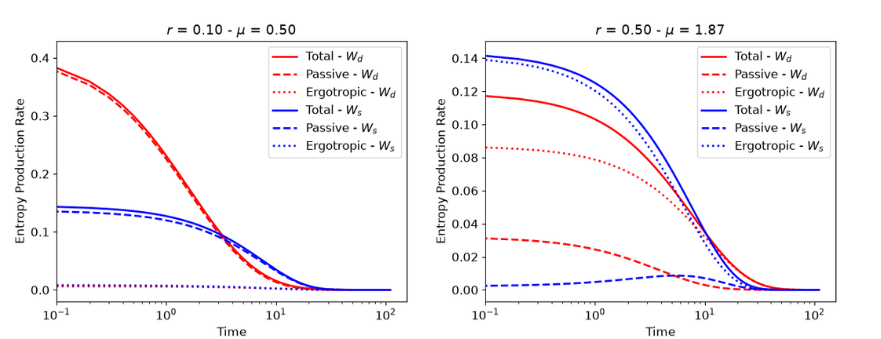
\includegraphics[width=\linewidth]{Images/Gaussian/Sprod-inversion-all.png}
    \caption{Left plot shows the entropy production rate of smaller $\mu$ and $r$. Right plot shows the entropy production rate of bigger $\mu$ and $r$. Heating the displaced state is in red and cooling the squeezed state is in blue. The passive contribution is in dashed lines, the ergotropic contribution is in dotted lines, and the total entropy production rate is in solid lines.}
    \label{fig:sprod-inversion}
\end{figure}

